\documentclass[]{book}
\usepackage{lmodern}
\usepackage{amssymb,amsmath}
\usepackage{ifxetex,ifluatex}
\usepackage{fixltx2e} % provides \textsubscript
\ifnum 0\ifxetex 1\fi\ifluatex 1\fi=0 % if pdftex
  \usepackage[T1]{fontenc}
  \usepackage[utf8]{inputenc}
\else % if luatex or xelatex
  \ifxetex
    \usepackage{mathspec}
  \else
    \usepackage{fontspec}
  \fi
  \defaultfontfeatures{Ligatures=TeX,Scale=MatchLowercase}
\fi
% use upquote if available, for straight quotes in verbatim environments
\IfFileExists{upquote.sty}{\usepackage{upquote}}{}
% use microtype if available
\IfFileExists{microtype.sty}{%
\usepackage{microtype}
\UseMicrotypeSet[protrusion]{basicmath} % disable protrusion for tt fonts
}{}
\usepackage[margin=1in]{geometry}
\usepackage{hyperref}
\hypersetup{unicode=true,
            pdftitle={Cours de Statistique et Probabilités},
            pdfauthor={FC},
            pdfborder={0 0 0},
            breaklinks=true}
\urlstyle{same}  % don't use monospace font for urls
\usepackage{natbib}
\bibliographystyle{apalike}
\usepackage{color}
\usepackage{fancyvrb}
\newcommand{\VerbBar}{|}
\newcommand{\VERB}{\Verb[commandchars=\\\{\}]}
\DefineVerbatimEnvironment{Highlighting}{Verbatim}{commandchars=\\\{\}}
% Add ',fontsize=\small' for more characters per line
\usepackage{framed}
\definecolor{shadecolor}{RGB}{248,248,248}
\newenvironment{Shaded}{\begin{snugshade}}{\end{snugshade}}
\newcommand{\KeywordTok}[1]{\textcolor[rgb]{0.13,0.29,0.53}{\textbf{{#1}}}}
\newcommand{\DataTypeTok}[1]{\textcolor[rgb]{0.13,0.29,0.53}{{#1}}}
\newcommand{\DecValTok}[1]{\textcolor[rgb]{0.00,0.00,0.81}{{#1}}}
\newcommand{\BaseNTok}[1]{\textcolor[rgb]{0.00,0.00,0.81}{{#1}}}
\newcommand{\FloatTok}[1]{\textcolor[rgb]{0.00,0.00,0.81}{{#1}}}
\newcommand{\ConstantTok}[1]{\textcolor[rgb]{0.00,0.00,0.00}{{#1}}}
\newcommand{\CharTok}[1]{\textcolor[rgb]{0.31,0.60,0.02}{{#1}}}
\newcommand{\SpecialCharTok}[1]{\textcolor[rgb]{0.00,0.00,0.00}{{#1}}}
\newcommand{\StringTok}[1]{\textcolor[rgb]{0.31,0.60,0.02}{{#1}}}
\newcommand{\VerbatimStringTok}[1]{\textcolor[rgb]{0.31,0.60,0.02}{{#1}}}
\newcommand{\SpecialStringTok}[1]{\textcolor[rgb]{0.31,0.60,0.02}{{#1}}}
\newcommand{\ImportTok}[1]{{#1}}
\newcommand{\CommentTok}[1]{\textcolor[rgb]{0.56,0.35,0.01}{\textit{{#1}}}}
\newcommand{\DocumentationTok}[1]{\textcolor[rgb]{0.56,0.35,0.01}{\textbf{\textit{{#1}}}}}
\newcommand{\AnnotationTok}[1]{\textcolor[rgb]{0.56,0.35,0.01}{\textbf{\textit{{#1}}}}}
\newcommand{\CommentVarTok}[1]{\textcolor[rgb]{0.56,0.35,0.01}{\textbf{\textit{{#1}}}}}
\newcommand{\OtherTok}[1]{\textcolor[rgb]{0.56,0.35,0.01}{{#1}}}
\newcommand{\FunctionTok}[1]{\textcolor[rgb]{0.00,0.00,0.00}{{#1}}}
\newcommand{\VariableTok}[1]{\textcolor[rgb]{0.00,0.00,0.00}{{#1}}}
\newcommand{\ControlFlowTok}[1]{\textcolor[rgb]{0.13,0.29,0.53}{\textbf{{#1}}}}
\newcommand{\OperatorTok}[1]{\textcolor[rgb]{0.81,0.36,0.00}{\textbf{{#1}}}}
\newcommand{\BuiltInTok}[1]{{#1}}
\newcommand{\ExtensionTok}[1]{{#1}}
\newcommand{\PreprocessorTok}[1]{\textcolor[rgb]{0.56,0.35,0.01}{\textit{{#1}}}}
\newcommand{\AttributeTok}[1]{\textcolor[rgb]{0.77,0.63,0.00}{{#1}}}
\newcommand{\RegionMarkerTok}[1]{{#1}}
\newcommand{\InformationTok}[1]{\textcolor[rgb]{0.56,0.35,0.01}{\textbf{\textit{{#1}}}}}
\newcommand{\WarningTok}[1]{\textcolor[rgb]{0.56,0.35,0.01}{\textbf{\textit{{#1}}}}}
\newcommand{\AlertTok}[1]{\textcolor[rgb]{0.94,0.16,0.16}{{#1}}}
\newcommand{\ErrorTok}[1]{\textcolor[rgb]{0.64,0.00,0.00}{\textbf{{#1}}}}
\newcommand{\NormalTok}[1]{{#1}}
\usepackage{longtable,booktabs}
\usepackage{graphicx,grffile}
\makeatletter
\def\maxwidth{\ifdim\Gin@nat@width>\linewidth\linewidth\else\Gin@nat@width\fi}
\def\maxheight{\ifdim\Gin@nat@height>\textheight\textheight\else\Gin@nat@height\fi}
\makeatother
% Scale images if necessary, so that they will not overflow the page
% margins by default, and it is still possible to overwrite the defaults
% using explicit options in \includegraphics[width, height, ...]{}
\setkeys{Gin}{width=\maxwidth,height=\maxheight,keepaspectratio}
\IfFileExists{parskip.sty}{%
\usepackage{parskip}
}{% else
\setlength{\parindent}{0pt}
\setlength{\parskip}{6pt plus 2pt minus 1pt}
}
\setlength{\emergencystretch}{3em}  % prevent overfull lines
\providecommand{\tightlist}{%
  \setlength{\itemsep}{0pt}\setlength{\parskip}{0pt}}
\setcounter{secnumdepth}{5}
% Redefines (sub)paragraphs to behave more like sections
\ifx\paragraph\undefined\else
\let\oldparagraph\paragraph
\renewcommand{\paragraph}[1]{\oldparagraph{#1}\mbox{}}
\fi
\ifx\subparagraph\undefined\else
\let\oldsubparagraph\subparagraph
\renewcommand{\subparagraph}[1]{\oldsubparagraph{#1}\mbox{}}
\fi

%%% Use protect on footnotes to avoid problems with footnotes in titles
\let\rmarkdownfootnote\footnote%
\def\footnote{\protect\rmarkdownfootnote}

%%% Change title format to be more compact
\usepackage{titling}

% Create subtitle command for use in maketitle
\newcommand{\subtitle}[1]{
  \posttitle{
    \begin{center}\large#1\end{center}
    }
}

\setlength{\droptitle}{-2em}
  \title{Cours de Statistique et Probabilités}
  \pretitle{\vspace{\droptitle}\centering\huge}
  \posttitle{\par}
  \author{FC}
  \preauthor{\centering\large\emph}
  \postauthor{\par}
  \date{}
  \predate{}\postdate{}

\usepackage{booktabs}
\usepackage{amsthm}
\makeatletter
\def\thm@space@setup{%
  \thm@preskip=8pt plus 2pt minus 4pt
  \thm@postskip=\thm@preskip
}
\makeatother

\usepackage{amsthm}
\newtheorem{theorem}{Theorem}[chapter]
\newtheorem{lemma}{Lemma}[chapter]
\theoremstyle{definition}
\newtheorem{definition}{Definition}[chapter]
\newtheorem{corollary}{Corollary}[chapter]
\newtheorem{proposition}{Proposition}[chapter]
\theoremstyle{definition}
\newtheorem{example}{Example}[chapter]
\theoremstyle{remark}
\newtheorem*{remark}{Remark}
\let\BeginKnitrBlock\begin \let\EndKnitrBlock\end
\begin{document}
\maketitle

{
\setcounter{tocdepth}{1}
\tableofcontents
}
\chapter{Préambule}\label{preambule}

Ce support de cours est largement inspiré du livre de Lafaye de Micheaux
et al. \cite{LAF} ainsi que du cours de Statistique de Bernard Ycart de
l'Université de Grenoble Alpes.

\chapter{Décrire une ou plusieurs séries de valeurs}\label{intro}

\section{Les graphiques}\label{les-graphiques}

Si la série de valeurs est qualitative on fera un diagramme en barres :
voir un exemple avec la figure 1.

Si la série de valeurs est quantitative :

\begin{itemize}
\tightlist
\item
  valeurs discrètes : diagramme en bâtons (voir figure 2)
\item
  valeurs continues : histogramme (voir figure 3)
\end{itemize}

\begin{figure}[htbp]
\centering
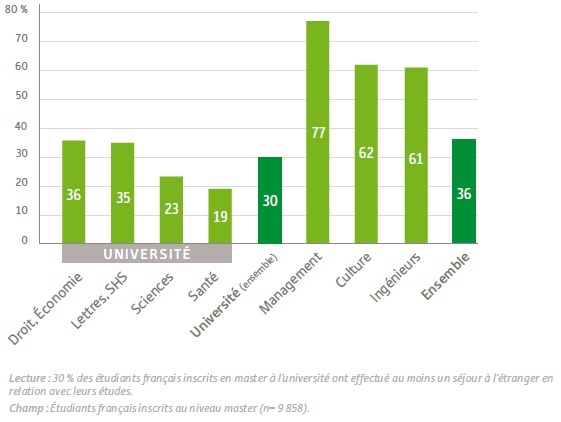
\includegraphics{./figures/figure1.jpg}
\caption{figure 1 : Diagramme en barres (source : Observatoire le vie
étudiante)}
\end{figure}

\begin{figure}[htbp]
\centering
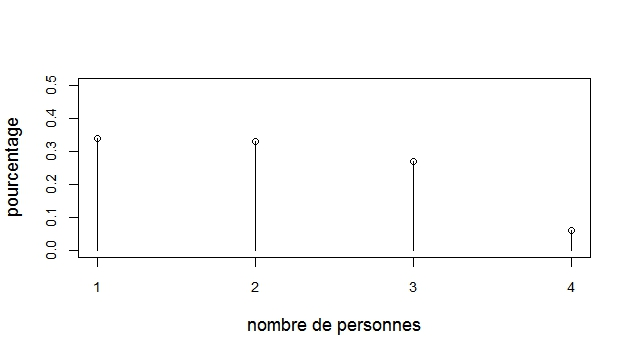
\includegraphics{./figures/figure2.jpg}
\caption{figure 2 : Diagramme en bâtons : nombre de personnes par ménage
en Rhône-Alpes au 01/01/2011 (source : INSEE)}
\end{figure}

\begin{figure}[htbp]
\centering
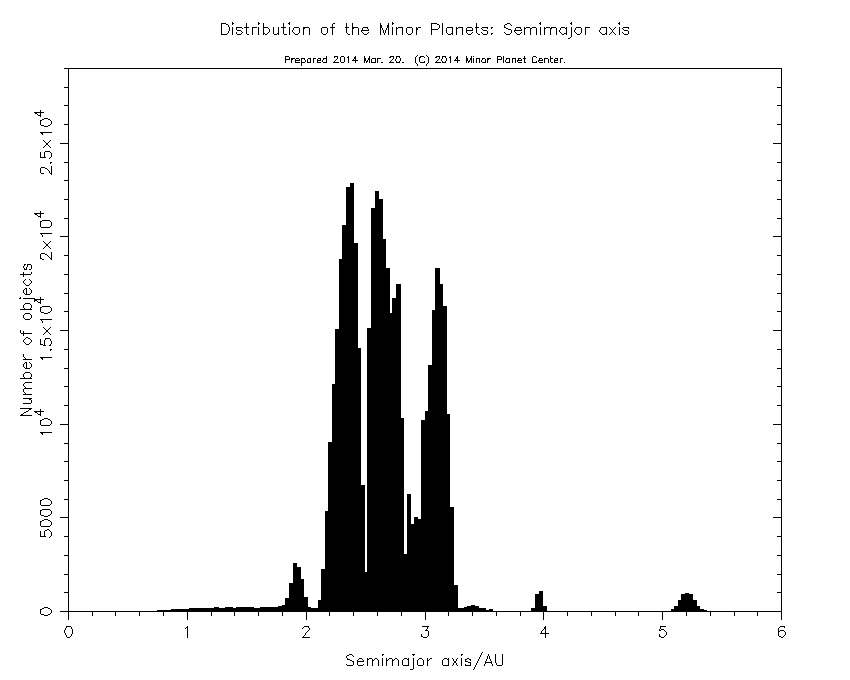
\includegraphics{./figures/figure3.jpg}
\caption{figure 3 : Histogramme : demi grands axes des orbites
d'astéroïdes (source : Minor Planet Center)}
\end{figure}

Pour les variables quantitatives, on peut aussi représenter la fonction
de répartition (empirique) notée \(\hat{F}(x)\): pour cela on calcule
pour chaque point de l'axe des \(x\) ainsi : (voir exemple figure 4)

\begin{align*}
\hat{F}(x)=\frac{ \text{nombre de valeurs dans la série}\leqslant x}{n}
\end{align*}

\begin{figure}[htbp]
\centering
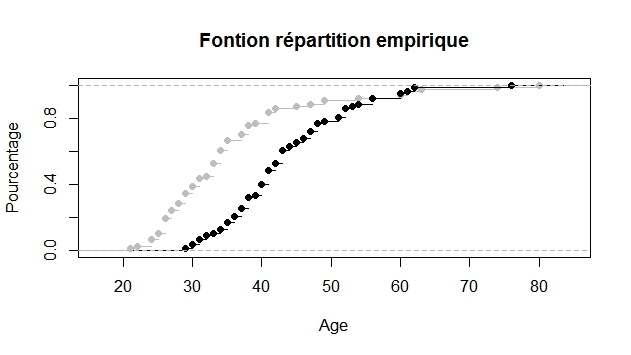
\includegraphics{./figures/figure4.jpg}
\caption{figure 4 : Fonction de répartition des âges des acteurs (en
noir) et actrices (en gris) ayant reçu l'oscar du meilleur acteur depuis
1929 (source : Journal of Statistics Education)}
\end{figure}

\section{Résumés numériques}\label{resumes-numeriques}

\subsection{Résumés de position d'une
distribution}\label{resumes-de-position-dune-distribution}

\subsubsection{Le ou les modes}\label{le-ou-les-modes}

Les modes sont les valeurs de la variable \(X\) qui apparaissent le plus
fréquemment. Il peuvent se calculer pour une variable de n'importe quel
type, bien que pour une variable continue, on parle de classe modale.

\subsubsection{La médiane}\label{la-mediane}

La médiane d'une série statistique est la valeur \(m_e\) de la variable
\(X\) qui partage cette série statistique en deux parties (inférieure et
supérieure à \(m_e\)) de même effectif. Cette quantité ne se calcule pas
sur des variables purement qualitatives. Pour la calculer, on distingue
deux cas :

\begin{itemize}
\item
  L'effectif total \(N\) est impair, alors \(m_e\) est la valeur située
  à la position \(\frac{N+1}{2}\)
\item
  L'effectif total \(N\) est pair, alors \(m_e\) est n'importe quelle
  valeur entre \(\frac N2\) et \(\frac N2 +1\).
\end{itemize}

\subsubsection{La moyenne}\label{la-moyenne}

Elle se calcule uniquement sur des variables quantitatives via la
fonction mean().

\subsubsection{Les fractiles}\label{les-fractiles}

Le fractile d'ordre \(p\) (\(0<p<1\)) est la valeur \(q_p\) de la
variable \(X\) qui coupe l'échantillon en deux portions, l'une ayant un
nombre d'éléments (inférieurs à \(q_p\)) égal à \(p\%\) du nombre total
d'éléments et l'autre à \((1-p)\%\) étant supérieurs à \(q_p\). Il ne se
calcule pas pour des variables purement qualitatives. Si on prend
\(p=0.5\), on retrouve la définition de la médiane.

\subsection{Résumé de dispersion d'une
distribution}\label{resume-de-dispersion-dune-distribution}

Ces résumés peuvent être calculés uniquement pour des variables
quantitatives. Les principales sont :

\begin{itemize}
\tightlist
\item
  Variance \(\sigma^2\) de la population.
\item
  l'écart type est la racine carrée de la variance.
\item
  Coefficient de variation \(c_v=\frac{\sigma}{\mu}\)
\end{itemize}

\chapter{Probabilités}\label{probabilites}

\section{Densité et fonction de répartition d'une variable quantitative
continue}\label{densite-et-fonction-de-repartition-dune-variable-quantitative-continue}

La variable aléatoire \(X\) associée à une fonction \(f\) donnée et
définie sur \(\mathbb{R}\) représente le fait de tirer un nombre au
hasard avec la probabilité suivante
:\[{\rm Proba}(X\leq t)=\int_{-\infty}^{t} f(x) dx = F(t)\] où \(t\) est
un réel fixé.

Naturellement, cette écriture n'a de sens que si :

\begin{enumerate}
\def\labelenumi{\arabic{enumi}.}
\item
  \(f\) est une fonction positive sur \(\mathbb{R}\)
\item
  \(\displaystyle\int_{-\infty}^{+\infty} f(x) dx=1\).
\end{enumerate}

\(f\) est appelée ``\textbf{densité}'' de \(X\).

Cette probabilité est notée \(F(t)\) : \(F\), vue comme une fonction de
\(t\) définie sur \(\mathbb{R}\), est appelée \textbf{fonction de
répartition} de \(X\). La valeur \(F(t)\) peut être vue comme l'aire de
la surface délimitée par la demi-droite \(]-\infty,t]\), la droite
\(y=t\) et la courbe représentative de \(f\).

\begin{itemize}
\tightlist
\item
  L'espérance de \(X\) (appelée aussi moyenne de \(X\)) correspond à la
  valeur suivante :
\end{itemize}

\[E(X)=\int_{-\infty}^{+\infty} xf(x)\,dx.\]

\begin{itemize}
\tightlist
\item
  La variance de \(X\) est :
\end{itemize}

\[{\rm Var}(X)=\mathbb E\left[ (X-\mathbb E[X])^2 \right]  = \mathbb E[X^2] - \mathbb E[X]^2 =  \int_{-\infty}^{+\infty}x^2f(x)\,dx-\mathbb E[X]^2.\]

\section{Exemple : la loi normale}\label{exemple-la-loi-normale}

On appelle loi normale la loi d'une variable aléatoire réelle continue
\(X\) dont la densité s'écrit :
\[f(x)=\frac{1}{\sigma\sqrt{2\pi}}e^{-\displaystyle\frac{1}{2}\frac{(x-\mu)^2}{\sigma^2}}\]
où \(\mu\) est la moyenne de \(X\) et \(\sigma^2\) est la variance de
\(X\). On dit que \(X\) suit la loi Normale de moyenne \(\mu\) et de
variance \(\sigma^2\) et on note \(X\leadsto \mathcal N(\mu,\sigma^2)\).

Si \(\mu=0\), on dit que \(X\) est centrée.

Si \(\sigma^2=1\), on dit que \(X\) est réduite.

Une propriété importante sur la loi normale est la suivante :

\BeginKnitrBlock{theorem}
\protect\hypertarget{thm:unnamed-chunk-1}{}{\label{thm:unnamed-chunk-1}}Si
\(X\leadsto \mathcal N(\mu,\sigma^2)\) alors
\(\displaystyle \frac{X-\mu}{\sigma} \leadsto \mathcal N(0,1)\).
\EndKnitrBlock{theorem}

Remarque : Attention ! Cette propriété nous dit que pour centrer et
réduire une loi normale, il faut lui retrancher sa moyenne et
\textbf{diviser par l'écart type (et non pas la variance)}.

Les figures suivantes nous donnent des exemples de densité de
différentes lois normales.

\begin{Shaded}
\begin{Highlighting}[]
\KeywordTok{curve}\NormalTok{(}\KeywordTok{dnorm}\NormalTok{(x,}\DecValTok{0}\NormalTok{,}\DecValTok{1}\NormalTok{),}\DataTypeTok{from =} \NormalTok{-}\DecValTok{5}\NormalTok{,}\DataTypeTok{to =} \DecValTok{7}\NormalTok{,}\DataTypeTok{col=}\StringTok{"red"}\NormalTok{,}\DataTypeTok{main=}\StringTok{"Densités de lois normales"}\NormalTok{,}\DataTypeTok{ylab=}\StringTok{"densité"}\NormalTok{)}
\KeywordTok{curve}\NormalTok{(}\KeywordTok{dnorm}\NormalTok{(x,}\DecValTok{0}\NormalTok{,}\DecValTok{2}\NormalTok{),}\DataTypeTok{from =} \NormalTok{-}\DecValTok{5}\NormalTok{,}\DataTypeTok{to =} \DecValTok{7}\NormalTok{,}\DataTypeTok{col=}\StringTok{"blue"}\NormalTok{,}\DataTypeTok{add =} \OtherTok{TRUE}\NormalTok{)}
\KeywordTok{curve}\NormalTok{(}\KeywordTok{dnorm}\NormalTok{(x,}\DecValTok{2}\NormalTok{,}\DecValTok{2}\NormalTok{),}\DataTypeTok{from =} \NormalTok{-}\DecValTok{5}\NormalTok{,}\DataTypeTok{to =} \DecValTok{7}\NormalTok{,}\DataTypeTok{col=}\StringTok{"green"}\NormalTok{,}\DataTypeTok{add =} \OtherTok{TRUE}\NormalTok{)}
\KeywordTok{legend}\NormalTok{(}\DecValTok{4}\NormalTok{,}\FloatTok{0.3}\NormalTok{,}\DataTypeTok{legend=}\KeywordTok{c}\NormalTok{(}\StringTok{"N(0,1)"}\NormalTok{,}\StringTok{"N(0,4)"}\NormalTok{,}\StringTok{"N(2,4)"}\NormalTok{),}\DataTypeTok{col =} \KeywordTok{c}\NormalTok{(}\StringTok{"red"}\NormalTok{,}\StringTok{"blue"}\NormalTok{,}\StringTok{"green"}\NormalTok{),}\DataTypeTok{lty=}\DecValTok{1}\NormalTok{)}
\end{Highlighting}
\end{Shaded}

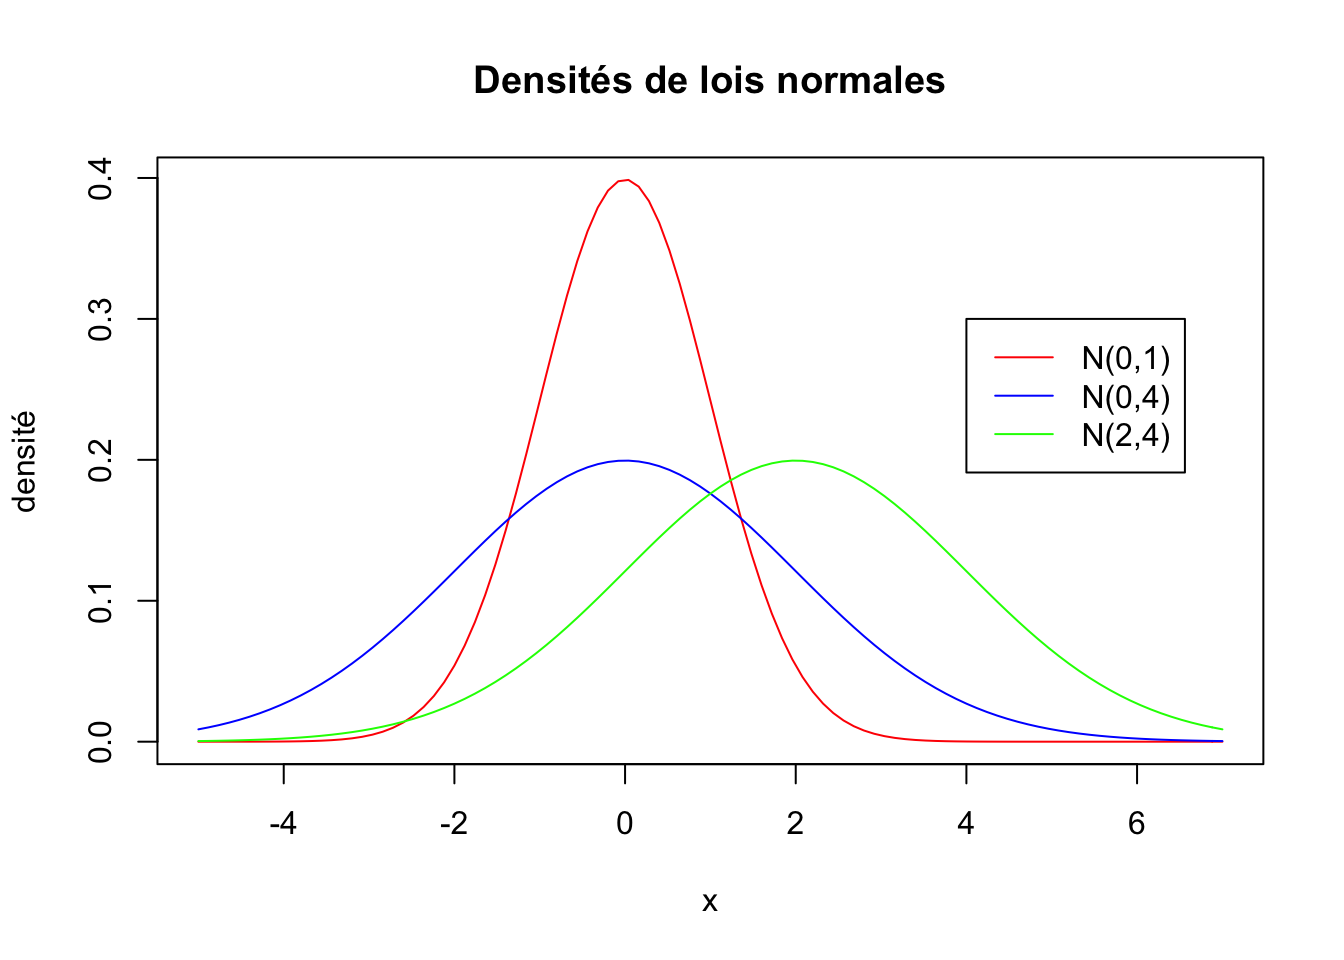
\includegraphics{bookdown-demo_files/figure-latex/unnamed-chunk-2-1.pdf}

\section{Loi forte des grands
nombres}\label{loi-forte-des-grands-nombres}

\section{Théorème central limite}\label{theoreme-central-limite}

Le théorème central limite dit que, si un grand nombre de variables
aléatoires indépendantes ayant la même loi sont ajoutées, leur somme
suit approximativement une loi normale.

\begin{enumerate}
\def\labelenumi{\arabic{enumi}.}
\item
  Pour des échantillons distribués suivant une loi binomiale, la loi
  binomiale \(B(n,p)\) se comporte comme la loi normale
  \(\mathcal N(np,np(1-p))\) pour \(n\) grand.
\item
  Si \(\{X_i\}_{i=1}^{\infty}\) est une suite de variables aléatoires
  indépendantes de même loi et de moyenne \(\mu\) et de variance
  \(\sigma^2\), alors
  \(\bar X_n=\frac{\displaystyle \sum_{i=1}^nX_i}{n}\) suit
  approximativement une loi normale \(\mathcal N(\mu,\sigma^2/n)\) pour
  \(n\) grand
\item
  ou, \(Z_n=\frac{\bar X_n-\mu}{\sigma/\sqrt{n}}\), variable centrée
  réduite issue de \(\bar X_n\), suit approximativement une loi normale
  \(\mathcal N(0,1)\) pour \(n\) grand.
\end{enumerate}

\chapter{Estimation}\label{estimation}

\section{Introduction}\label{introduction}

\textbf{En probabilités, on travaille avec une loi connue. En
statistique, cette loi est inconnue.}

Le statisticien travaille sur des données (notes de qualité de pièces
produites dans une usine, données météorologiques, résultats
d'expériences médicales ou physiques,\ldots{}). Il le fait à la demande
d'un interlocuteur qui a des attentes plus ou moins précises. Ces
attentes peuvent être de plusieurs types :

\begin{itemize}
\tightlist
\item
  extraire des résumés pertinents des données,
\item
  répondre à une question comme ``le réchauffement climatique est-il
  réel ?'',
\item
  prendre une décision comme la mise sur le marché d'un nouveau
  médicament,
\item
  effectuer une prévision, par exemple sur le résultat d'une élection
  qui aura lieu prochainement,\ldots{}
\end{itemize}

Il élabore un modèle et construit des outils pour répondre aux questions
de son interlocuteur dans ce modèle. Il doit bien sûr garder un sens
critique vis à vis du modèle qu'il a construit. Il est bien sûr crucial
pour le statisticien d'estimer les paramètres au vu des données dont il
dispose et d'avoir une idée de la précision de cette estimation. On
introduit tout d'abord les estimateurs puis on verra enfin comment
évaluer la précision des estimateurs au travers d'intervalles de
confiance.

En résumé, voici les étapes de la statistique inférentielle :

\begin{enumerate}
\def\labelenumi{\arabic{enumi}.}
\item
  Observation d'une variable \(X\) sur un groupe d'individus choisis
  d'une façon aléatoire et indépendante dans la population totale.
\item
  On obtient des observations \(x_1, \ldots,x_n\), réalisations de
  variables aléatoires indépendantes et de même loi \(X_1,\ldots,X_n\).
  On fait une étude descriptive de \(x_1, \ldots,x_n\) (histogramme,
  moyenne, \(\ldots\)).
\item
  Au vu de l'étude descriptive, trouver une loi de probabilité
  acceptable pour les variables \(X_1, \ldots,X_n\).
\item
  Inférence statistique : utiliser \(x_1, \ldots,x_n\) pour estimer les
  paramètres du modèle et en déduire des propriétés sur la population
  totale.
\end{enumerate}

\section{Statistique et estimateur}\label{statistique-et-estimateur}

\begin{enumerate}
\def\labelenumi{\arabic{enumi}.}
\tightlist
\item
  Pour un paramètre inconnu, un estimateur est une fonction des données,
  prenant des valeurs proches de ce paramètre.
\end{enumerate}

1 Avant que les données ne soient collectées, l'estimateur est une
variable aléatoire 2 Une fois les données collectées, l'estimation est
la valeur de l'estimateur pour ces données.

\begin{enumerate}
\def\labelenumi{\arabic{enumi}.}
\setcounter{enumi}{1}
\tightlist
\item
  Estimer un paramètre \(\theta\) inconnu, c'est donc trouver une
  statistique \(T=\tau(X_1,\ldots,X_n)\) dont on pense que la valeur
  observée \(\tau(x_1,\ldots,x_n)\) sera probablement ``suffisamment
  proche'' de la valeur inconnue \(\theta\).
\end{enumerate}

Dans ce cas, \(T\) sera appelé estimateur de \(\theta\), et,
\(\tau(x_1,\ldots,x_n)\) sera une estimation de \(\theta\). (valeur
numérique).

\begin{enumerate}
\def\labelenumi{\arabic{enumi}.}
\tightlist
\item
  Le biais de \(T\) est la différence entre l'espérance de \(T\) et la
  vraie valeur (inconnue) de \(\theta\) : Biais=\(\mathbb E[T]-\theta\).
\item
  L'erreur quadratique est l'espérance des carrés des différences : QE=
  \(\mathbb E[(T-\theta)^2]\).
\end{enumerate}

L'estimateur \(T\) est :

\begin{itemize}
\tightlist
\item
  sans biais si le biais est nul (Les valeurs de \(T\) sont centrées sur
  la vraie valeur)
\item
  asymptotiquement sans biais si le biais tend vers 0 quand la taille de
  l'échantillon tend vers l'infini.
\item
  consistant si la probabilité de s'éloigner de la valeur à estimer de
  plus de \(\epsilon\) (\(\epsilon\) petit) tend vers 0 quand la taille
  de l'échantillon augmente.
\end{itemize}

Voici maintenant quelques exemples standards d'estimateurs

\begin{enumerate}
\def\labelenumi{\arabic{enumi}.}
\item
  La fréquence empirique d'un évènement est un estimateur sans biais
  consistant de la probabilité de cet évènement.
\item
  La moyenne empirique d'un échantillon est un estimateur sans biais
  consistant de l'espérance théorique de ces variables :
  \[T(X_1,\ldots,X_n)=\bar
  X=\frac{1}{n}\displaystyle\sum_{i=1}^nX_i\]
\item
  La variance empirique notée \(S_n^2\) d'un échantillon (lorsque la
  moyenne est inconnue) est
\end{enumerate}

\[
S_n^2=\frac{1}{n}\displaystyle\sum_{i=1}^n(X_i-\bar X)^2 .
\]

Cet estimateur est biaisé. On peut montrer que

\[
\mathbb E [S_n^2] = \frac{n-1}{n} \sigma^2
\]

Ainsi, on obtient un estimateur sans biais en multipliant la variance
empirique par \(n/(n-1)\) où \(n\) désigne la taille de l'échantillon,
noté \({S_n^\prime}^2\) :

\[
{S^\prime_n}^2=\frac{1}{n-1}\displaystyle\sum_{i=1}^n(X_i-\bar X)^2 .
\]

C'est cette dernière quantité qui est donnée dans le logiciel R via la
fonction var(). Si l'on veut calculer la variance empirique d'un
échantillon sous le logiciel R, il faudra donc faire le nécessaire : par
exemple faire une nouvelle fonction que l'on pourra appeler var.pop().

\section{Estimation par intervalle de
confiance}\label{estimation-par-intervalle-de-confiance}

Lorsque l'on estime un paramètre \(\theta\), on veut avoir une idée de
la précision de l'estimation effectuée. C'est le rôle des intervalles de
confiance.

\textbf{Problème} :

Peut-on trouver deux statistiques \(T_1\) et \(T_2\) telles que
\[p(T_1\leq \theta\leq T_2)=1-\alpha\] avec \(0<\alpha<1\) fixé ? ou
encore peut-on trouver deux statistiques \(T_1\) et \(T_2\) de manière à
ce qu'on ait beaucoup de chance de trouver le paramètre inconnu entre
ces deux statistiques ?

\begin{enumerate}
\def\labelenumi{\arabic{enumi}.}
\tightlist
\item
  L'intervalle \([T_1, T_2]\) est un intervalle aléatoire appelé
  intervalle de confiance.
\item
  \(\alpha\) est le risque d'erreur. Le paramètre \(\alpha\) représente
  la probabilité que l'intervalle
  \([T_1(X_1,\ldots,X_n), T_2(X_1,\ldots,X_n)]\) ne contienne pas le
  paramètre inconnu \(\theta\). En affirmant que \([T_1, T_2]\) contient
  \(\theta\), on se trompe en moyenne 100\(\alpha\) fois sur 100.
\item
  \((1-\alpha)\) est appelé niveau de confiance ou coefficient de
  sécurité.
\end{enumerate}

\subsection{Intervalles de confiance pour une
moyenne}\label{intervalles-de-confiance-pour-une-moyenne}

\subsubsection{Cas d'un échantillon
gaussien}\label{cas-dun-echantillon-gaussien}

On suppose que \(X\) suit une loi normale \(\mathcal N(\mu,\sigma^2)\).
On rappelle que la moyenne empirique et que la variance empirique sont
données par
\[\bar X=\frac{1}{n}\displaystyle\sum_{i=1}^nX_i\quad{\rm and}\quad S^2=\frac{1}{n}\displaystyle\sum_{i=1}^n(X_i-\bar X)^2.\]

\begin{enumerate}
\def\labelenumi{\arabic{enumi}.}
\item
  Si \(\sigma^2\) est connue, un intervalle de confiance de niveau
  \(1-\alpha\) pour la moyenne \(\mu\) est
  \[\left[ \bar X - u_{1-\alpha/2} \frac{\sigma}{\sqrt{n}};\bar X + u_{1-\alpha/2} \frac{\sigma}{\sqrt{n}} \right]\]
  où \(u_{1-\alpha/2}\) est le quantile d'ordre \(1-\alpha/2\) de la loi
  normale \(\mathcal N(0,1)\).
\item
  Si \(\sigma^2\) est inconnue, un intervalle de confiance de niveau
  \(1-\alpha\) pour la moyenne \(\mu\) est
\end{enumerate}

\[
\left[\bar X - t_{1-\alpha/2} \frac{S}{\sqrt{n}};\bar X + t_{1-\alpha/2} \frac{S}{\sqrt{n}} \right]
\]

où \(t_{1-\alpha/2}\) est le quantile d'ordre \(1-\alpha/2\) de la loi
de Student de paramètre \(n-1\).

\subsubsection{Cas d'un échantillon non gaussien, mais de grande
taille}\label{cas-dun-echantillon-non-gaussien-mais-de-grande-taille}

Pour de grands échantillons, sans hypothèse de normalité, un intervalle
de confiance de niveau \(1-\alpha\) pour la moyenne \(\mu\) est

\[
\left[\bar X - u_{1-\alpha/2} \frac{S}{\sqrt{n}};\bar X + u_{1-\alpha/2} \frac{S}{\sqrt{n}} \right]
\] où \(u_{1-\alpha/2}\) est le quantile d'ordre \(1-\alpha/2\) de la
loi normale \(\mathcal N(0,1)\).

\subsection{Intervalle de confiance pour une
variance}\label{intervalle-de-confiance-pour-une-variance}

On se place dans le cas où \(X\) suit une loi normale,
\(\mathcal N(\mu,\sigma^2)\).

Un intervalle de confiance de niveau \(1-\alpha\) pour la variance
\(\sigma^2\) est

\[
\left[ \frac{nS^2}{q^{n-1}_{1-\alpha/2}};\frac{nS^2}{q^{n-1}_{\alpha/2}}\right] = \left[ \frac{(n-1)(S^\prime)^2}{q^{n-1}_{1-\alpha/2}};\frac{(n-1)(S^\prime)^2}{q^{n-1}_{\alpha/2}}\right] 
\]

où \(q^{n-1}_{1-\alpha/2}\) est le quantile d'ordre \(1-\alpha/2\) de la
loi du chi-2 de paramètre \(n-1\) et \(q^{n-1}_{\alpha/2}\) son quantile
d'ordre \(\alpha/2\).

\subsection{Intervalle de confiance pour une
proportion}\label{intervalle-de-confiance-pour-une-proportion}

On suppose que l'on est en présence d'un échantillon de grande taille
(en pratique \(n\geq 30\)). Un intervalle de confiance de niveau
\((1-\alpha)\) pour une proportion \(p\) inconnue est

\[
\left[\bar X - u_{1-\alpha/2} \sqrt{(\frac{\hat X (1-\hat X)}{n})};\hat X + u_{1-\alpha/2} \sqrt{(\frac{\hat X (1-\hat X)}{n})} \right].
\]

où \(n\) est la taille de l'échantillon, \(\bar X\) la fréquence
empirique et \(u_{1-\alpha/2}\) est le quantile d'ordre \(1-\alpha/2\)
de la loi normale \(\mathcal N(0,1)\).

\chapter{Tests}\label{tests}

\bibliography{packages.bib,book.bib}


\end{document}
